\documentclass[journal,onecolumn]{IEEEtran}

\title{Applied Spatial and Temporal Data Analysis}
\author{ Vijay K. Shah}

\usepackage{amsmath}
\usepackage{mathtools}
\usepackage{graphicx}
\usepackage{enumitem}
\usepackage{epsfig}
\usepackage{color}
\usepackage{algorithm}
\usepackage[noend]{algpseudocode}
\usepackage{subfigure}
\usepackage[justification=centering]{caption}
\usepackage{csvsimple}
\usepackage{longtable}

\begin{document}
\maketitle

\section{\textbf{Data Retrieval}}

\textit{Q 1. Find 100 CNN news articles online (try to find them in different categories, e.g., sports and
finance). You need to find the new article by yourself. Pls ignore picture or other non-text data
in the new article.} \\

In this section, I first describe how 100 CNN News links were retrieved followed by the discussion on data retrieval from each link. \textbf{Note:} I actually crawled 200 CNN News articles for this assignment.

\subsection{\underline{100 CNN News Link Retrieval}:}

\begin{itemize}[label={}]
\item \textbf{Step 1:} I downloaded the urls for all the articles in the webpage - http://www.cnn.com/US/archive/

\item \textbf{Step 2:} I stored them in a text file \textbf{links.txt} in home folder \textbf{helloProject}. 

\end{itemize}
Step 1 and 2 are handled by script file \textbf{cnn\_spider.py} stored in folder \textbf{helloProject/helloProject/Spiders/}


\subsection{\underline{Data (Articles) Retrieval from all links}:}

I created a script \textbf{pages\_spider.py} to navigate through all urls (stored in links.txt) and download the content body using Scrappy request. Here, I used Scrapy selector.xpath('//p/text()') ,  selector.xpath('//h/text()') and  selector.xpath('//span/text()') so that only useful texts are downloaded instead of entire html file. After that, I only consider alphabetical words with atleast 3 alphabets using a regrex [a-zA-Z]$\{3,\}$ \\


\textbf{Note: } The script \textbf{pages\_spider.py} can be found in folder "helloProject/helloProject/Spiders"
Each downloaded article is stored as article- \textbf{article\_\%Article-headerName\%.txt} in folder \textbf{Articles/}


\begin{figure}[h]
\begin{center}
 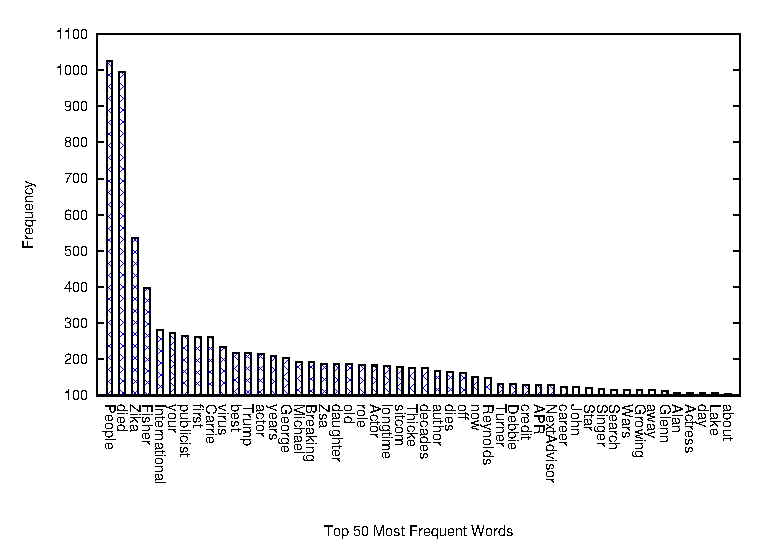
\includegraphics[width = 6.5in, height = 3.5 in] {Plots/wordFreq_allArticles.eps}
 \caption {Frequency vs Top K features (most frequent) }
 \end{center}
\end{figure}



\section{\textbf{Feature Selection}}
\textit{Q 2. Convert them to data matrix (each row is an article and each column is a unique term).}\\

In this section, I present the details of forming a data matrix where each row is an article and each column is a unique word.

\subsection{\underline{Creation of data matrix}}

\begin{itemize}[label={}]

\item \textbf{Step 1: }  I filtered out insignificant words from the data retrieved from each article as discussed in Homework 1.

\item \textbf{Step 2:} I sorted out the list of words in decreasing order of its frequency. (only until I get first  top K frequent unique words).

\item \textbf{Step 3:} I created a data matrix of size (Number of Articles) X (Top K Most Frequent Words). Each cell contains the frequency of each unique word (Column) for following article (Row).

\end{itemize} 

\subsection{\underline{Addition of \textit{Category} Column to the data matrix}}

I have added a new column called \textit{Category}, which represents the category of the article (row). The category list is as follows:
\begin{itemize}
\item \textbf{entertainment} %(86 articles)
\item \textbf{us } %(15 articles)
\item \textbf{health} % (33 articles)
\item \textbf{politics} % (11 articles)
\item \textbf{opinions}% (30 articles)
\end{itemize}

\iffalse
\begin{table}
\scriptsize
\centering
\caption {List of Categories}  \label{Category}
\begin{tabular}{|c|} 
\hline % inserts single horizontal line
entertainment \\
\hline
 us \\
 \hline
 health \\
 \hline
 politics \\
 \hline
 opinions\\
\hline
\end{tabular}
\end{table}
\fi


\section{Clustering with different Similarity Metrics}
\textit{Q 3. Run K-means clustering with Euclidean, Cosine and Jaccard similarity. (Specify K as the number of categories of your 100 CNN news articles)}


\subsection{K-Means with Euclidean Distance}
We have run K-means clustering with Euclidean Distance taking (i) 3 features and (ii) 9 features as shown in Fig. 2 and Table I respectively.

\begin{figure}[h] \label{euclid_default}
\begin{center}
 \includegraphics[scale=.70] {Plots/euclid_default.eps}
 \caption { Euclidean Distance (with 3 features)}
 \end{center}
\end{figure}

\csvautotabular{EuclideanDefaultGeneral/euclideanDefaultCentroids.csv} 
{Table I: Euclidean Distance (with 9 features) \label{euclid_default_10}


\subsection{K-Means with Euclidean Similarity}
We have run K-means clustering with Euclidean Similarity taking (i) 3 features and (ii) 9 features as shown in Fig. 3 and Table II respectively.

\textbf{Computation of Euclidean Similarity}: For a pair of articles say, Article(i) = $\{w_{i0}, w_{i1}, \dots w_{i(K-1)} \}$ and Article(j) = $\{w_{j0}, w_{j1}, \dots w_{j(K-1)} \}$, the euclidean similarity $E(ij)$ is given by

\begin{equation} \label{euclid_sim_eq}
E(ij) = \frac{1}{1 + \sqrt{(Article(i) - Article(j))^2}}
\end{equation}

\begin{figure}[h] \label{euclid_sim}
\begin{center}
 \includegraphics[scale=.70] {Plots/euclid_sim.eps}
 \caption { Euclidean Similarity (with 3 features)}
 \end{center}
\end{figure}

\csvautotabular{EuclideanSimilarityGeneral/euclideanSimCentroids.csv}
{Table II: Euclidean Similarity (with 9 features) \label{euclid_sim_10}}

\subsection{K-Means with Cosine Similarity}
We have run K-means clustering with Cosine Similarity taking (i) 3 features and (ii) 9 features as shown in Fig. 4 and Table III respectively.

\textbf{Computation of Cosine Similarity}: For a pair of articles say, Article(i) = $\{w_{i0}, w_{i1}, \dots w_{i(K-1)} \}$ and Article(j) = $\{w_{j0}, w_{j1}, \dots w_{j(K-1)} \}$, the cosine similarity $C(ij)$ is given by

\begin{equation} \label{cosine_sim_eq}
E(ij) = \frac{Article(i) Article(j)}{||Article(i)|| . ||Article(j)||}
\end{equation}

\begin{figure}[h] \label{cosine_sim}
\begin{center}
 \includegraphics[scale=.70] {Plots/cosine_sim.eps}
 \caption { Cosine Similarity (with 3 features)}
 \end{center}
\end{figure}

\csvautotabular{CosineSimilarityGeneral/cosineSimCentroids.csv}
{Table III: Cosine Similarity (with 9 features) \label{cosine_sim_10}}

\subsection{K-Means with Jaccard Similarity}
We have run K-means clustering with Jaccard Similarity taking (i) 3 features and (ii) 9 features as shown in Fig. 5 and Table IV respectively.

\textbf{Computation of Jaccard Similarity}: For a pair of articles say, Article(i) = $\{w_{i0}, w_{i1}, \dots w_{i(K-1)} \}$ and Article(j) = $\{w_{j0}, w_{j1}, \dots w_{j(K-1)} \}$, the jaccard similarity $J(ij)$ is given by

\begin{equation} \label{jaccard}
J(ij) = \frac{Article(i) \cap Article(j)}{Article(i) \cup Article(j)}
\end{equation}


\begin{figure}[h] \label{jaccard_sim}
\begin{center}
 \includegraphics[scale=.70] {Plots/jaccard_sim.eps}
 \caption { Jaccard Similarity (with 3 features)}
 \end{center}
\end{figure}

\csvautotabular{JaccardSimilarityGeneral/jaccardSimCentroids.csv}
{Table IV: Jaccard Similarity (with 9 features) \label{jaccard_sim_10}}


\iffalse
\begin{figure}[h]
\begin{center}
 \includegraphics[scale=0.4] {Plots/f1Score.png}
 \caption {Precision/Recall} \label{precision}
 \end{center}
\end{figure}
\fi

\section{Evaluation of K-means with SSE}
\textit{Q 4. Evaluate K-means clustering results with SSE}

We evaluate K-means clustering against different metrics with SSE for following cases (i) 3 features (ii) 9 features and (iii) 50 features.

\begin{table}[h]
\begin{center}
\begin{tabular}{|c|c|c|c| } 

\hline % inserts single horizontal line
Metrics & SSE (3 features) & SSE ( 9  features) & SSE (50 features)\\
\hline
Euclidean Distance & 270.074074074 & 13279.4824897 & 14386.9788434(5 clusters) \\ \hline
Euclidean Similarity & 133.046 & 2.077 & 1.425 (2 clusters)\\ \hline
Cosine Similarity & inf & inf  & 149.869 (4 clusters)\\ \hline
Jaccard Similarity & inf & 103.001 & 101.11 (4 clusters) \\ \hline

\hline %inserts single line
\end{tabular}
\end{center}
%\label{table:nonlin} % is used to refer this table in the text
\end{table}
Table V: Evaluation with K-Means against different Metrics 


\section{Analysis}
As aforementioned, there are basically 2 clusters for dataset with 3 features, detected by all of above similarity metrics. Whereas with 9 features, Euclidean distance is able to detect upto 4 clusters (close to original 5 clusters (categories)). However, with 50 features, all 5 clusters were determined by euclidean distance. The cosine and jaccard similarity metrics also yield upto 4 clusters. Among similarity metrics, the SSE is least for euclidean similarity.

However, it is evident that the euclidean distance performs the clustering best. It may be because the distance between any two point is significant in case of euclidean distance, hence easily distinguishable to be assigned to a certain closest centroid. Also, it requires least number of iterations to converge compared to other metrics (i.e. similarity metrics).

\end{document}